\begin{block}{Parameter Estimation in Latent Variable Models}
  \begin{center}
  \begin{tikzpicture}[scale=2.0]
    \drawgen{(0,0)};
    \node[below=0.1cm of x.south] {Generative Models};
    \drawdisc{(4,0)};
    \node[below=0.1cm of y.south] {Discriminative Models};
  \end{tikzpicture}
  \end{center}
  \vspace{-2ex}
  \begin{itemize}
    \item Latent variable models (LVMs) are hard to learn because latent
      variables introduce non-convexities in the log-likelihood
      function.
    \item In practice, local methods (EM, gradient descent, etc.) are
      employed, but these can stuck in local optima.
    \item {\bf Can we develop efficient consistent estimators for discriminative latent variable models?}
      \begin{itemize}
        \item Why discriminative LVMs? Easy to add features, often more accurate.
        \item The method of moments has been used for consistent parameter estimation in several generative LVMs, e.g. HMMs${}^1$, LDA${}^1$, and stochastic block models${}^2$.
        \item Can we extend these techniques to discriminative LVMs?
      \end{itemize}
    \item {\bf Main result}: Consistent estimator for a simple discriminative model; the mixture of linear regressions.
      \begin{itemize}
        \item {\bf Key Idea:} Expose tensor factorization structure using regression.
        \item {\bf Theory:} We prove polynomial sample and computational complexity.
      \end{itemize}
  \end{itemize}              
  \footnotesize{%
    \hfill
    [1] Anandkumar, Hsu, Kakade, 2012; [2] Anandkumar, Ge, Hsu, Kakade, 2012
    }
\end{block}

%\vfill

\begin{block}{Aside: Tensor Operations}
  \vspace{-3ex}
  \splitcolumn{%
    \begin{itemize}
      \item Tensor Product
        \begin{align*}
          x\tp{3}       &= x \otimes x \otimes x \\
          x\tp{3}_{ijk} &= x_i x_j x_k
        \end{align*}
      \item Inner product
        \begin{align*}
          \innerp{A}{B} &= \sum_{ijk} A_{ijk} B_{ijk} \\
            &= \innerp{\vvec{A}}{\vvec{B}} 
        \end{align*}
    \end{itemize}
  }{%
  \begin{tikzpicture}[scale=1.3]
    \point{tensoring-pos}{(0,0)}
    % Tensoring
    \tikzcube{tensoring}{black,fill=white}{($(tensoring-pos) + (0cm,-1.0cm) + (0,0,0)$)}{1}{1}{1};
    \node at ($(tensoring) + (1.0cm,-0.3cm)$) {$=$};
    \tikzcube{v1}{black,fill=white}{($(tensoring) + (2.5cm,-0.3cm)$)}{1}{0.3}{0.3};
    \node (lbl1) at ($(v1) + (0.40cm,-0.1cm)$) {$\times$};
    \tikzcube{v2}{black,fill=white}{($(v1) + (1cm,0.3cm)$)}{0.3}{1}{0.3};
    \node at ($(lbl1) + (1cm,0.0cm)$) {$\times$};
    \tikzcube{v3}{black,fill=white}{($(v2) + (1cm,-0.3cm)$)}{0.3}{0.3}{1};

    % Inner product
    \point{ptA}{(0cm,-3.0cm)}
    \point{ptB}{($(ptA) + (2cm,0)$)}

    \tikzcube{innerpA}{black,fill=yellow}{($(ptA) + (0,0,0)$)}{1}{1}{1};
    \tikzcube{innerpB}{black,fill=blue!70}{($(ptB) + (0,0,0)$)}{1}{1}{1};

    \innerpdiagt{(ptA)}{(ptB)};
    \node[scale=1.0] at ($(ptB) + (1.5cm,-0.3cm)$) {$= \mathmg{0.5}$};

    % Inner product 2
    \point{ptvA}{($(ptA) + (0,-2cm)$)}
    \point{ptvB}{($(ptB) + (0,-2cm)$)}

    \tikzrect{innerpAv}{black,fill=yellow}{($(ptvA) + (0,0.5cm)$)}{0.3}{2.0};
    \tikzrect{innerpBv}{black,fill=blue!70}{($(ptvB) + (0,0.5cm)$)}{0.3}{2.0};

    \innerpdiagt{(ptvA)}{(ptvB)};
    \node[scale=1.0] at ($(ptvB) + (1.5cm,-0.3cm)$) {$= \mathmg{0.5}$};
  \end{tikzpicture}
  }
\end{block}

%\vfill

\begin{block}{Mixture of Linear Regressions}
  \begin{columns}[onlytextwidth]
    \begin{column}{0.55\textwidth}
      \begin{tikzpicture}
        \point{mark}{(0,0)}
        \drawdisc{(5cm,0)}
      \end{tikzpicture}
      \begin{itemize}
        \item For a particular $x$, we draw $y$ as follows,
        \begin{itemize}
          \item $h \sim \Mult([\pi_1, \pi_2, \cdots, \pi_k])$.
          \item $y = \beta_h^T x + \epsilon$.
        \end{itemize}
      \end{itemize}
    \end{column}
    \hfill
    \begin{column}{0.45\textwidth}
        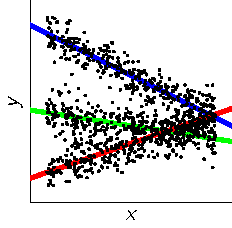
\includegraphics[width=7cm,height=8cm,keepaspectratio]{figures/mlr-5.pdf}
    \end{column}
  \end{columns}

  \begin{itemize}
    \item Given $\mathcal{D} = \{(x_i,y_i)\}_{i=1}^n$, we want to recover the parameters $\pi$ and $B$.
  \begin{tikzpicture}[scale=0.7]
    \node[anchor=east] (data) at (-2cm,0) {%
    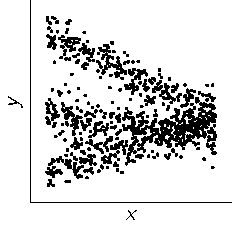
\includegraphics[width=6cm,height=7cm,keepaspectratio]{figures/mlr-6.pdf}
    };

    % x, y
    \node[anchor=west,scale=1.0] (params) at (1.5cm,0) {%
      $\begin{bmatrix} \pi_1 \\ \pi_2 \\ \vdots \\ \pi_k \end{bmatrix}  
        \ub{
       \begin{bmatrix} 
                 &         &       &         \\
                 &         &       &         \\
         \beta_1 & \beta_2 & \dots & \beta_k \\
                 &         &       &         \\
                 &         &       &         
               \end{bmatrix}}_{B} $
      };
    %\node[anchor=west,right=0.1cm of params] {%
    %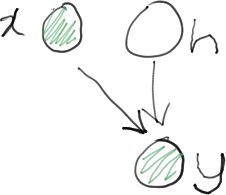
\includegraphics[width=4cm,height=2cm,keepaspectratio]{figures/disc.png}
    %};

    \draw[-latex] (data) -- node[above]{?} (params);
  \end{tikzpicture}

  \item Our approach uses low-rank regression to reduce the problem to tensor eigendecomposition. 
  \begin{tikzpicture}[scale=1.8]
    \spectralexpertsdiag
    \node[style=txt] at (reg-label) {low-rank regression};
    \node[style=txt] at (tf-label) {tensor factorization};

    %\point{reg-assumptions}{($(reg-label) - (0cm,1.0cm)$)};
    %\node[style=txt] (assumptions) at (data3 |- reg-assumptions) {%
    %  %{\bf Assumptions:}
    %};
    %\node[style=txt] at (reg-assumptions) {%
    %    %$\begin{aligned}
    %    %  \hat\E[\vvec(x\tp{2})\tp{2}] &\succ 0\\
    %    %  \hat\E[\vvec(x\tp{3})\tp{2}] &\succ 0.
    %    %\end{aligned}$
    %    };
    %\node[style=txt] (tf-assumptions) at ($(reg-assumptions.west) + (1em,0)$) {%
    %    %$\begin{aligned}
    %    %  \pi &\succ 0\\
    %    %  rank(B) &= k \le d
    %    %\end{aligned}$
    %    };
    \node[style=txt,below=0.1em of reg-label] (reg-compl) {%
      $O\left( k\ 
      \hlmath{blue}{\|x\|^{12}}
      \hlmath{DarkGreen}{\|\beta\|^{6}}
      \hlmath{red}{\|\E[\epsilon^2]\|^{6}}
      \right)$};
    \node[style=txt,below=0.1em of tf-label] {%
    $O\left( \frac{k \pi_{\max}^2}{\sigma_k(M_2)^5} \right)$};

    \node[scale=0.8,style=txt, left=0.1em of reg-compl] {%
      {\bf Sample Complexity:}
    };

  \end{tikzpicture}
  \end{itemize}

  \vspace{-1ex}

\end{block}

